\documentclass[11pt]{article}

\usepackage{fullpage}
\usepackage{amsmath}
\usepackage{amssymb}
\usepackage{amsthm}
\usepackage{fancyhdr}
\usepackage{algorithm}
\usepackage{algorithmic}
\usepackage{bm}
\usepackage{listings}
\usepackage{graphicx}
\usepackage{caption2}
\usepackage{subfigure}
\usepackage{float}
\usepackage{extpfeil}
\usepackage{color}
\usepackage[usenames,dvipsnames]{xcolor}


\newtheorem{theorem}{Theorem}[section]
\newtheorem{lemma}[theorem]{Lemma}
\newtheorem{corollary}[theorem]{Corollary}
\newtheorem{proposition}[theorem]{Proposition}
\newtheorem{definition}[theorem]{Definition}
\newtheorem{conjecture}[theorem]{Conjecture}
\newtheorem{remark}[subsection]{Remark}

%%
\newcommand\numberthis{\addtocounter{equation}{1}\tag{\theequation}}

%% define new symbols
\def\bx{\bm{x}}
\def\bb{\bm{b}}
\def\ba{\bm{a}}
\def\bc{\bm{c}}
\def\bf{\bm{f}}
\def\by{\bm{y}}
\def\bu{\bm{u}}
\def\bv{\bm{v}}
\def\BW{\bm{W}}
\def\BA{\bm{A}}
\def\bz{\bm{z}}
\def\BZ{\bm{Z}}
\def\BH{\bm{H}}
\def\BL{\bm{L}}
\def\BU{\bm{U}}
\def\BV{\bm{V}}
\def\BB{\bm{B}}
\def\BC{\bm{C}}
\def\BD{\bm{D}}
\def\BE{\bm{E}}
\def\BW{\bm{W}}
\def\BQ{\bm{Q}}
\def\BG{\bm{G}}
\def\BA{\bm{A}}
\def\BX{\bm{X}}
\def\BY{\bm{Y}}
\def\BQ{\bm{Q}}
\def\BI{\bm{I}}
\def\BR{\bm{R}}

%% define new brackets
\def\la{\left\langle}
\def\ra{\right\rangle}
\def\ln{\left\|}
\def\rn{\right\|}
\def\lb{\left(}
\def\rb{\right)}
\def\lsb{\left[}
\def\rsb{\right]}
\def\lcb{\left\{}
\def\rcb{\right\}}

%%
\DeclareMathOperator*{\argmin}{arg\,min}
\DeclareMathOperator*{\argmax}{arg\,max}

%%
\title{Homework II}
\author{Name: Shao Yanjun, Number: 19307110036}


\begin{document}
\maketitle

%------------------------------------
\begin{abstract}
This is Daniel's homework of  "Numerical Algorithms with Case Studies II".
\end{abstract}
%-------------------------------------
%=====================
\section{Problems}
\paragraph{Q1}
First of all, we have to embed the four chemistry equations into mathematical equations, where $(x_1,x_2,x_3,x_4)=(ln([H^+]),ln([OH^-]),ln([HCO_3^-]),ln([CO_3^{2-}]))$,
\begin{equation}
	\left\{
\begin{aligned}
	f_1(x)&=x_1+x_2-lg(10^{-14})=0\\
	f_2(x)&=x_1+x_3-lg(10^{-13.76})=0\\
	f_3(x)&=x_1-x_3+x_4\\
	f_4(x)&=lg(e^{x_1})-lg(e^{x_2}+e^(x_3)+2e^{x_4})
\end{aligned}
\right.
\end{equation}
Then, in order to use Newton method $x_{k+1}=-J^{-1}f(x_k)+x_k$, we need to compute the Jacobian matrix.
\begin{align}
J&=\begin{pmatrix}
	\frac{\partial f_1}{\partial x_1}&
	\frac{\partial f_1}{\partial x_2}&
	\frac{\partial f_1}{\partial x_3}&
	\frac{\partial f_1}{\partial x_4}\\
	\frac{\partial f_2}{\partial x_1}&
	\frac{\partial f_2}{\partial x_2}&
	\frac{\partial f_2}{\partial x_3}&
	\frac{\partial f_2}{\partial x_4}\\
	\frac{\partial f_3}{\partial x_1}&
	\frac{\partial f_3}{\partial x_2}&
	\frac{\partial f_3}{\partial x_3}&
	\frac{\partial f_3}{\partial x_4}\\
	\frac{\partial f_4}{\partial x_1}&
	\frac{\partial f_4}{\partial x_2}&
	\frac{\partial f_4}{\partial x_3}&
	\frac{\partial f_4}{\partial x_4}\\
\end{pmatrix}\\&=
\begin{pmatrix}
	1& 1& 0& 0\\
	1& 0& 1& 0\\
	1& 0& -1& 1\\
	1& -\frac{e^{x_2}}{e^{x_2}+e^{x_3}+2e^{x_4}}&
	-\frac{e^{x_3}}{e^{x_2}+e^{x_3}+2e^{x_4}}&
	-\frac{2e^{x_4}}{e^{x_2}+e^{x_3}+2e^{x_4}}
\end{pmatrix}
\end{align}
After several iteration, we finally find the pH of the rainwater, which is approximately $5.592643$.
\paragraph{Q2}
Sine function is perfectly interpolated with Lagrange method if $x$ is not too faraway from our taken points of $sin(x)$.
\begin{figure}[H]
	\centering
	\subfigure[interpolation of sin(x)]{
		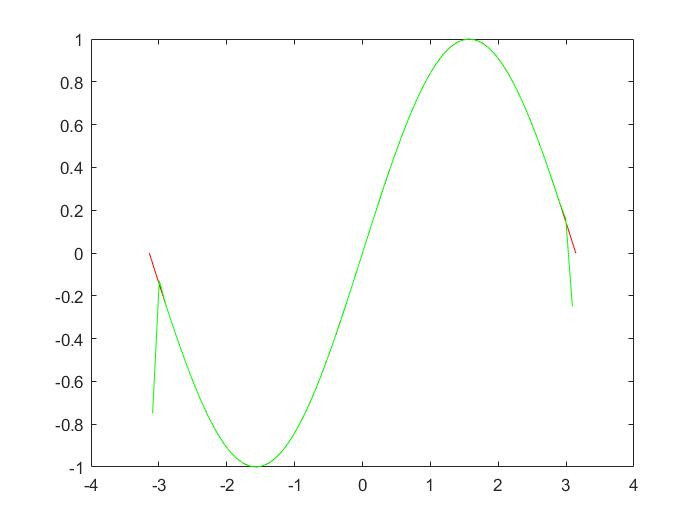
\includegraphics[width=0.4\linewidth]{interpolation_of_sin.jpg}
	}
	\subfigure[relative error]{
		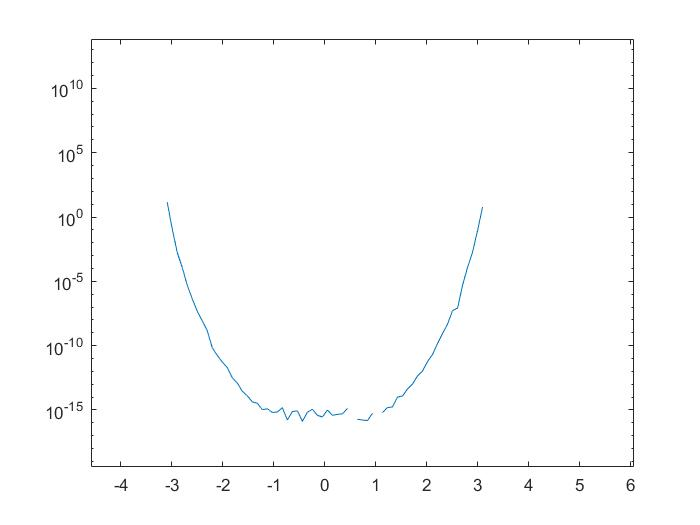
\includegraphics[width=0.4\linewidth]{relative_error_of_interpolation.jpg}
	}
\end{figure}
As we can see, the marginal points seem fit poorly, but the rest of them fits in fairly well.\\
\hspace*{0.4cm}
Secondly, we apply similar method to $f(x)=(1+25x^2)^{-1}$, the result remains good on limited range of points with the polynomial. While we start to estimate $x$ on marginal points, the result is terribly disappointing.
\begin{figure}[H]
	\centering
	\subfigure[interpolation of f(x)]{
		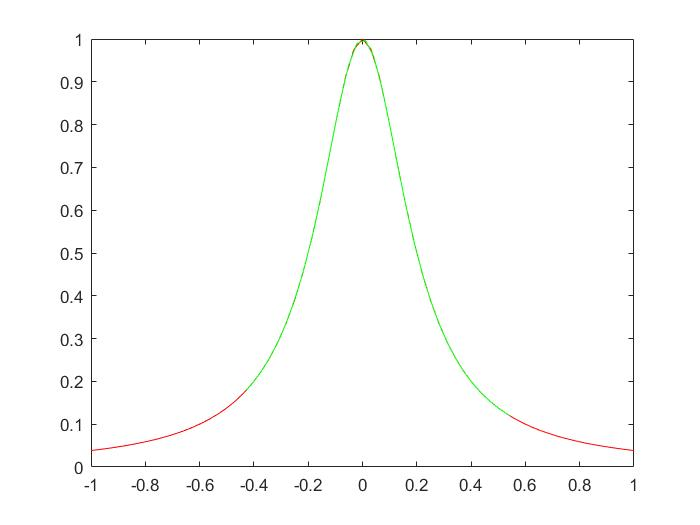
\includegraphics[width=0.4\linewidth]{interpolation_of_fx.jpg}
	}
	\subfigure[bad estimation]{
		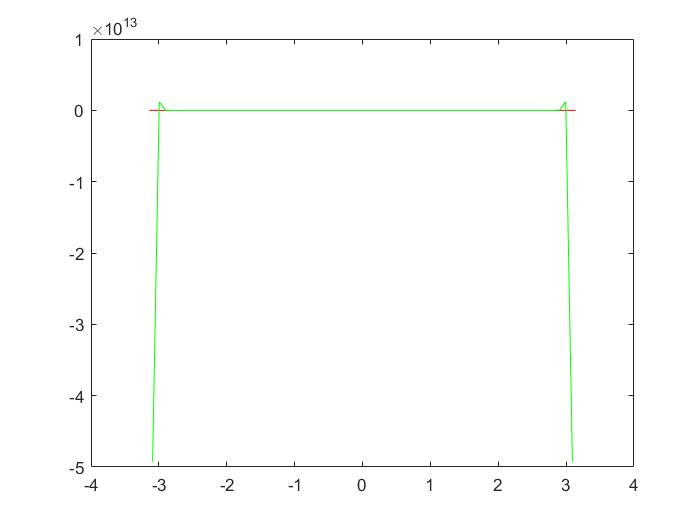
\includegraphics[width=0.4\linewidth]{bad_one.jpg}
	}
	\subfigure[bad estimation]{
		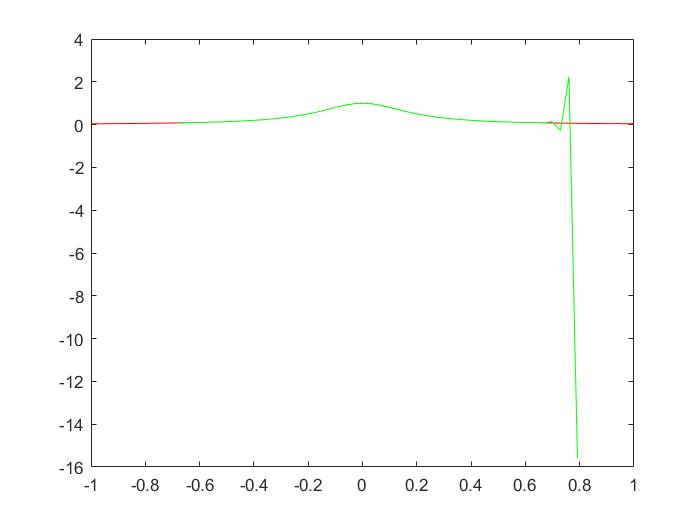
\includegraphics[width=0.4\linewidth]{bad_two.jpg}
	}
	\subfigure[relative error]{
		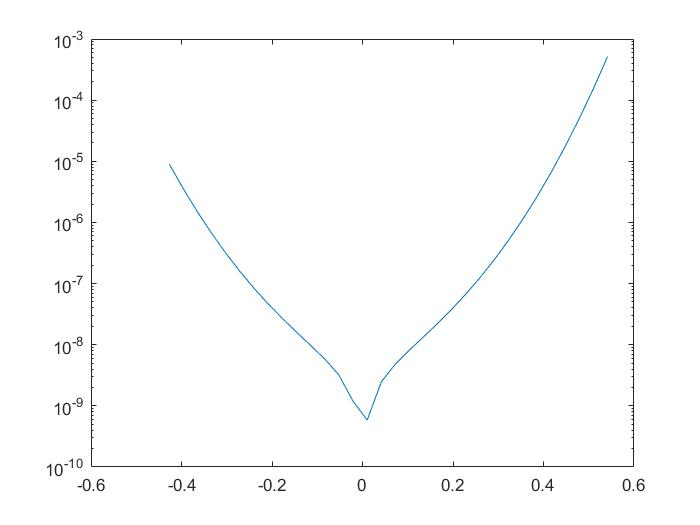
\includegraphics[width=0.4\linewidth]{relative_error_of_interpolation_fx.jpg}
	}
\end{figure}
\paragraph{Q3}
We can determine an n-degree polynomial with at least n+1 given points, and for n+1 consecutive integer points $(i,f(i)),(i+1,f(i+1)),\cdots,(i+n,f(i+n)) \in \mathbb{Z}$, we construct our lagrange polynomial as follows,
\begin{align}
	p(x)&=f(i)\frac{\prod_{j\ne i}(x-x_j)}{\prod_{j\ne k}(x_j-x_k)}+\cdots+f(i+n)\frac{\prod_{j\ne i+n}(x-x_j)}{\prod_{j\ne k}(x_j-x_k)}\\
	&=\sum_{k=0}^{n}(f(n+k)\cdot\frac{\prod_{j=i}^{n}(x-x_j)}{x-x_k}\cdot\frac{(-1)^{n-k}}{k!(n-k)!})
\end{align}
Put in $x=i+n+1$, we have,
\begin{align}
	p(i+n+1)&=\sum_{k=0}^{n}(f(n+k)\cdot\frac{(n+1)!}{n-k+1}\cdot\frac{(-1)^{n-k}}{k!(n-k)!})\\
	&=\sum_{k=0}^{n}((-1)^{n-k}f(n+k)\cdot\frac{(n+1)!}{k!(n-k+1)!})\\
	&=\sum_{k=0}^{n}(-1)^{n-k}\binom{n+1}{k}f(n+k)
\end{align}
Since $\forall k$, $\binom{n+1}{k}\in \mathbb{Z}$ is a combinatorial number, we have the aggregate of integers,
\begin{align}
	p(i+n+1)=\sum_{k=0}^{n}(-1)^{n-k}\binom{n+1}{k}f(n+k) \in \mathbb{Z}
\end{align}
Similarly, we can prove that $p(i+n+2), p(i+n+3) \cdots \in \mathbb{Z}$ through mathematical induction (i.e. given that we have been convinced already $(j,f(j)),(j+1,f(j+1)),\cdots,(j+n,f(j+n)) \in \mathbb{Z}$ for some $j>i$). And likewise, $\forall j<i$, we could still prove $p(j) \in \mathbb{Z}$ with the same method. 
%-------------------------------------
%=====================
\end{document}
